\documentclass{beamer}
\usetheme{Boadilla}

\usepackage{tikz}
\usetikzlibrary{shapes}

\title{Git Gud}
\author{Neil Ashford}
\institute{UQ Computing Society}
\date{2018-04-23T17:30+10:00}

\AtBeginSection[]
{
    \begin{frame}
        \frametitle{Outline}
        \tableofcontents[currentsection]
    \end{frame}
}

\begin{document}

\begin{frame}
    \titlepage
\end{frame}

\section{Introduction}

\subsection{Who am I}
\begin{frame}
    \frametitle{Who am I}
    \begin{itemize}[<+->]
        \item Neil Ashford
        \item 4th year Software\only<2->{\footnote{ish}} Engineering
        \item Committee member
        \item \texttt{@artemis} on slack, \url{ashfordneil0@gmail.com}
    \end{itemize}
\end{frame}

\subsection{What is this talk}
\begin{frame}
    \frametitle{What is this talk}
    Target Audience
    \pause
    \begin{itemize}[<+->]
        \item People who have never used version control.
        \item People who have ``memorised 5 shell commands and trust them implicitly without understanding''
    \end{itemize}
    \pause
    What I'll Cover
    \begin{itemize}[<+->]
        \item Some really basic version control you're familiar with, and its flaws.
        \item The pieces of a mental model of proper version control.
        \item How git represents each of those pieces to you.
        \item Flaws with git, and alternatives.
    \end{itemize}
\end{frame}

\section{The Version Control We Know}

\subsection{Meet the Culprit}
\begin{frame}
    \frametitle{Meet the Culprit}
    \begin{itemize}[<+->]
        \item Live demos suck, so we're trying to stick with something familiar.
        \item Please welcome our old friend...
        \item Microsoft Word\only<3->{\footnote{Okay I'm on a mac so it's pages but still}}
    \end{itemize}
\end{frame}

\subsection{Undo / Reverts}
\begin{frame}
    \frametitle{Undo / Reverts}

    \centering
    \begin{columns}
        \begin{column}{0.5\textwidth}
            \begin{itemize}[<+->]
                    \pause
                \item Type ``Hello''
                \item Type ``World''
                \item Type ``Filler Text''
                \item Press Undo
                \item Press Redo
                \item Press Undo again
            \end{itemize}
        \end{column}
        \begin{column}{0.5\textwidth}
            \begin{tikzpicture}
                \only<2->{
                    \node[circle, draw, minimum size=1cm] (A) at (0,0) {Hello};
                }
                \only<3->{
                    \node[circle, draw, minimum size=1cm] (B) at (0,-2) {World};
                    \draw[->] (A) -- (B);
                }
                \only<4,6>{
                    \node[circle, draw, minimum size=1cm] (C) at (0,-4) {Filler Text};
                    \draw [->] (B) -- (C);
                }
                \only<5,7>{
                    \node[gray, dashed, circle, draw, minimum size=1cm] (C) at (0,-4) {Filler Text};
                    \draw [gray, dashed, ->] (B) -- (C);
                }
            \end{tikzpicture}
        \end{column}
    \end{columns}

\end{frame}

\end{document}
